\section{Results}


\begin{figure}
	\centering
	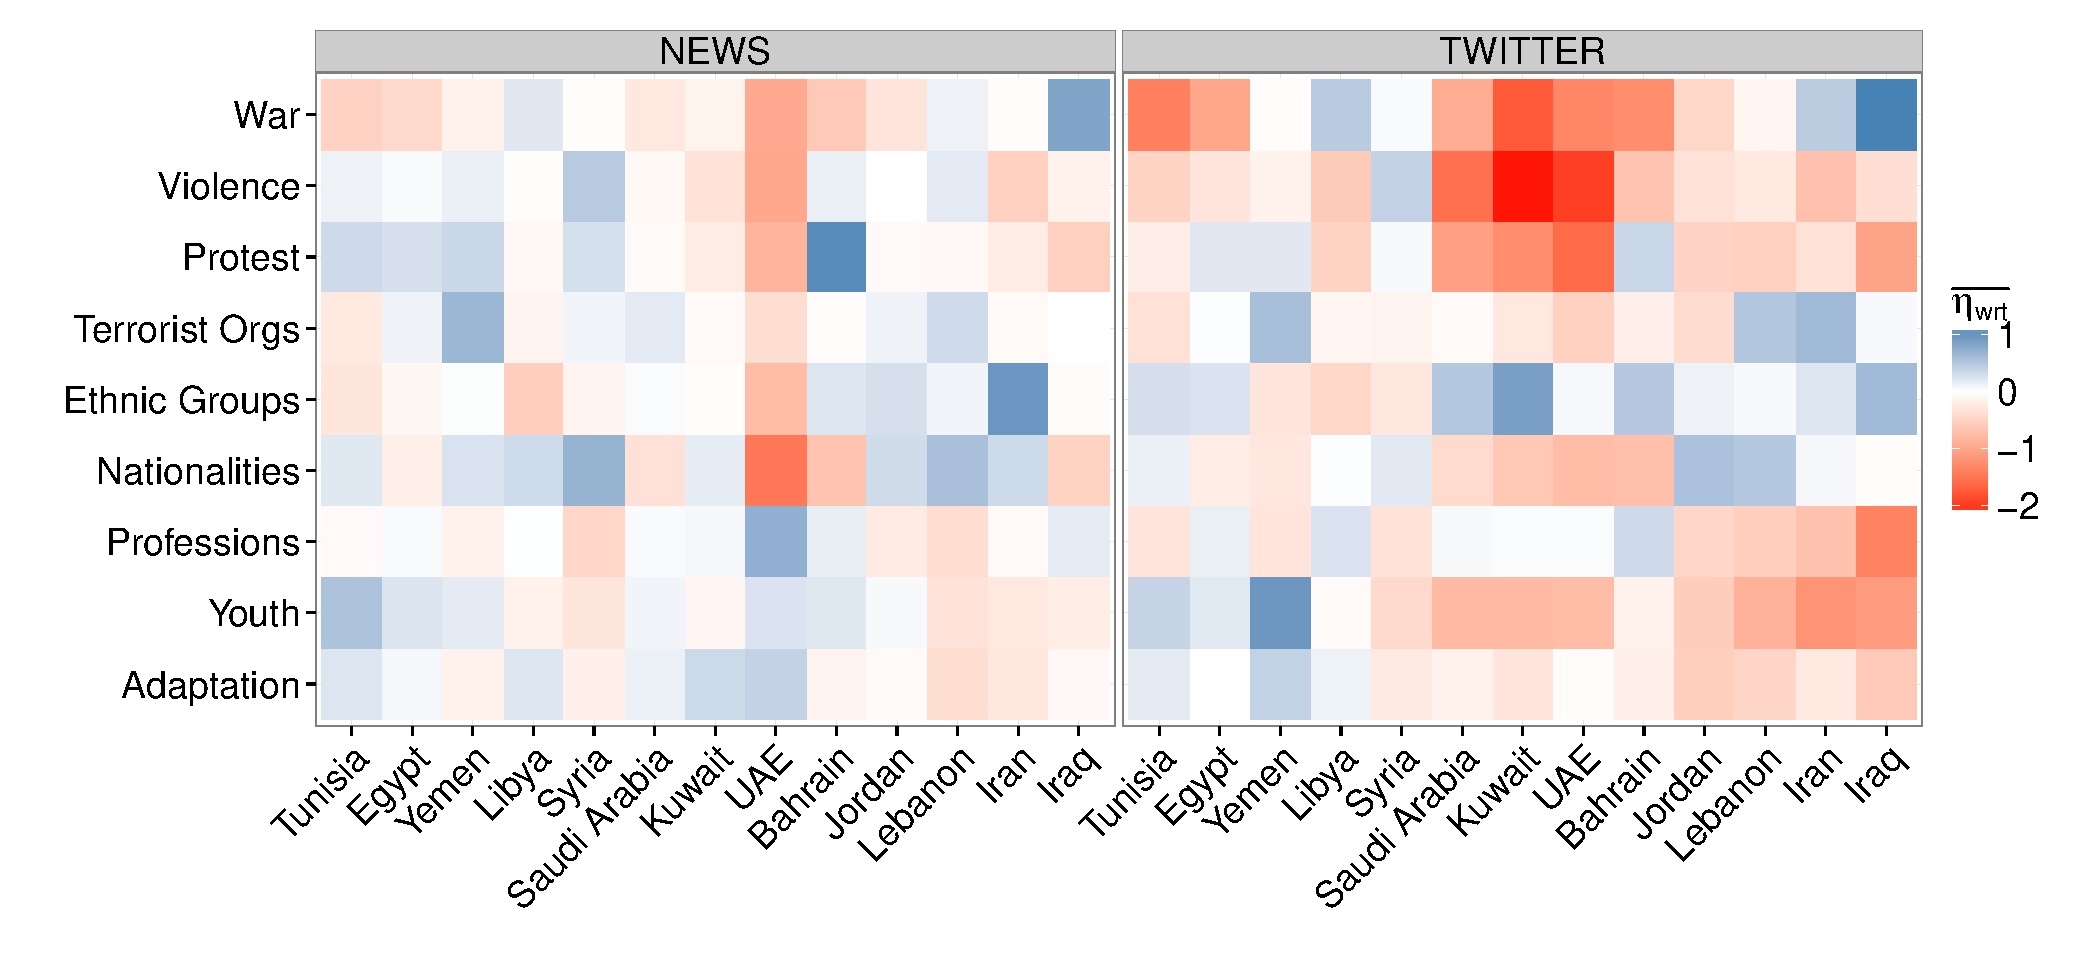
\includegraphics[width=\textwidth]{imgs/activity_topics}

	\caption{}
	\label{fig:overall}
\end{figure}

Figure \ref{fig:overall} shows the average level of activation across countries, per category of interest.  A few things are of interest.  First, Twitter looks more variable.  Second, similarities across categories. 

\begin{figure}
	\centering
	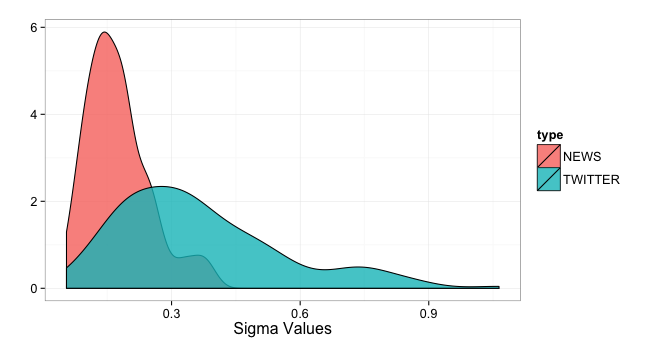
\includegraphics[width=.7\textwidth]{imgs/diff_sigma}

	\caption{Distribution of Sigmas}
	\label{fig:sig}
\end{figure}

Figure \ref{fig:sig} shows that the Twitter data is more variable than the news data. This is what we would expect because ...  This tells us also that changes in distributions on Twitter may not necessarily be as interesting as changes in the news data.

What about correlations?  That is, were news and Twitter correlated?  We cant use our data as is, BC non-IID.  But because estimates from the model are, bydefinition, AR(1), we can subtract off mean of the last month and then treat the result as IID.  Now we ask, given a country and a category, are these two time series independent? 


What about categories? Which were most correlated?

What about countries?

Where did the biggest jumps happen? Was that in accordance with anything?

% latex table generated in R 3.1.2 by xtable 1.7-4 package
% Wed May 13 14:32:55 2015
% latex table generated in R 3.1.2 by xtable 1.7-4 package
% Wed May 13 14:34:17 2015
\begin{table}[ht]
\centering
\begin{tabular}{rllllrr}
  \hline
 & category & country & type & date & val & sigma \\ 
  \hline
1 & war & syria & NEWS & 2011-03-01 & -0.72 & 0.18 \\ 
  2 & protest & syria & NEWS & 2011-03-01 & 1.02 & 0.27 \\ 
  3 & tribe & uae & TWITTER & 2012-10-01 & 1.55 & 0.42 \\ 
  4 & protest & tunisia & TWITTER & 2012-08-01 & 1.83 & 0.50 \\ 
  5 & war & lebanon & NEWS & 2011-03-01 & -0.64 & 0.18 \\ 
  6 & adaptation & libya & TWITTER & 2012-08-01 & 1.43 & 0.41 \\ 
  7 & adaptation & tunisia & TWITTER & 2011-10-01 & -1.42 & 0.41 \\ 
  8 & terrorist\_org & libya & NEWS & 2012-09-01 & 0.47 & 0.14 \\ 
  9 & terrorist\_org & egypt & TWITTER & 2012-11-01 & 0.72 & 0.21 \\ 
  10 & profession & libya & TWITTER & 2012-09-01 & -1.16 & 0.34 \\ 
   \hline
\end{tabular}
\end{table}
%
%	\item {\bf RQ1:} How did the topical focii of our news and Twitter data differ over time and across different nations?
%	\item {\bf RQ2:} How did (un)successful government overthrows change the topical focii of news and Twitter data?
%	\item {\bf RQ3:} Can we develop new hypotheses based on our data for the relationship between topical focii in news and Twitter data and (a lack of) social change? a holistic view of the topical focii of 